\documentclass[10pt,letterpaper]{article}
\usepackage[lmargin=2.2in,rmargin=0.7in,tmargin=1.0in,bmargin=1.0in]{geometry}
\usepackage{notes}
\begin{document}

\begin{center}
\Large\textbf{3.1 -- Definition, Linearity, and Transforms of Basic Functions}\\
\normalsize (Section 3.1)
\end{center}


%%%%%%%%%%%%%%%%%%%%%%%%%%%%%%%%%%%%
\section{Definition of the Laplace Transform}

% ---------------

\subsection{Definitions}
The \textbf{Laplace transform} converts a function of time into a function of the variable $s$. Let $x(t)$ be a function defined for $t \ge 0$. The Laplace transform of $x(t)$ is
\[
\boxed{
\mathcal{L}[x(t)] =  \int_0^\infty x(t)e^{-st}\,dt = X(s)
}
\]
Let's parse this equation. $x(t)$ is the input, the function we want to transform. $\mathcal{L}[\cdot]$ is the symbol for the Laplace transform. $X(s)$ is the transformed version of $x(t)$. The definition involves an integral with an $\infty$ in the limit. 

Notice that the integrand has two variables $s$ and $t$. It is a partial integral (which you learned in Calculus III). Partial integrals always eliminate the dummy variable, e.g.
$$
\int_0^1 \underbrace{(2x +3y)}_{\text{contains }x\text{ and }y}\,dx=\left(x^2+3xy)\right|_0^1 = \underbrace{1+3y}_{\text{only } y}.
$$
The Laplace transform changes a function of $t$ into a function of $s$ through partial integration:
\[
\mathcal{L}[\underbrace{x(t)}_{\text{only t}}] =  \underbrace{\int_0^\infty \underbrace{x(t)e^{-st}}_{\text{has both $s$ and $t$} }\,dt}_{\text{partial integral over }t} = \underbrace{X(s)}_{\text{only }s}
\]
When we integrate with respect to $t$, the variable $t$ disappears and the result becomes a function of $s$. The originals $t$ and $x$ are called \textbf{time domain variables}. The resulting $s$ and $X$ are called \textbf{transform domain variables}. 

% ---------------

\subsection{Improper Integral} 
The Laplace transform is actually an \textit{improper} integral because it has infinity in the upper limit. An \textbf{improper integral} over an unbounded interval is defined to be
$$
\int_a^\infty f(t)\,dt := \lim_{A \to \infty} \int_a^A f(t)\,dt =\lim_{A\to\infty}F(A)-F(a).
$$
If the limit exists, we say the improper integral \textbf{converges}. Otherwise, we say it \textbf{diverges}. For example, the integral of $1/t$ diverges because
$$
    \int_1^\infty \frac1t\,dt = \lim_{A\to\infty} (\ln A) - \ln1 = \infty.
$$
Suppose the integrand contains a parameter $p$, for example $f(t) = t^p$. The convergence of the improper integral depends on the value of $p$:
$$
    \int_1^\infty t^p\,dt = \lim_{A\to\infty} \frac{A^{p+1}}{p+1} - \frac{1}{p+1} = -\frac{1}{p+1}, \quad \text{if } p+1<0.
$$
We require $p+1$ to be negative so the term $A^{p+1}$ vanishes at infinity.
In a similar way, the existence of the transform 
$$
\mathcal{L}[x(t)] =  \int_0^\infty x(t)e^{-st}\,dt
$$
may depend on the value of $s$.

%%%%%%%%%%%%%%%%%%%%%%%%%%%%%%%%%%%%
\section{Transforms of Basic Funcions}

\subsection{Fundamental Examples}
In this section, we will directly use the definition of the Laplace transform to calculate the transform of three fundamental functions:
\begin{enumerate}
    \item Constant $x(t)=1$
    \item Exponential $x(t)=e^{at}$
    \item Linear $x(t)=t$
\end{enumerate}
Let's start with the constant.

\begin{example}[1]{
Compute the Laplace transform of $x(t)=1$ using the definition.
}
 By definition, we have
\[
\mathcal{L}[1] =\int_0^\infty (1)\,e^{-st}\,dt = \lim_{A\to\infty} \int_0^A e^{-st}\,dt.
\]
Evaluate the integral 
\[
\lim_{A\to\infty} \int_0^A e^{-st}\,dt= \lim_{A\to\infty} \left[-\frac{1}{s}e^{-st}\right]_0^A=-\frac{1}{s}\lim_{A\to\infty}(e^{-sA}-1).
\]
We want the limit as $A\to\infty$ to converge.
If $s<0$, then the limit is unbounded, so the improper integral \textit{diverges}. But if $s>0$ then we have 
\[
-\frac{1}{s}\lim_{A\to\infty}(e^{-sA}-1) = -\frac{1}{s}(0-1)= \frac1s.
\]
The transform of the constant is
\[
\boxed{\mathcal{L}\{1\}=\frac{1}{s},\quad s>0.}
\]
\end{example}

%%%%%%%%%%%%%%%%%%%%%%%%%%%%%%%%%%%%

\begin{example}[2]{
Compute the Laplace transform of $x(t)=e^{at}$ using the definition, where $a$ is a constant.
}
We start with the definition 
\[
\mathcal{L}[e^{at}]=\int_0^\infty e^{at}e^{-st}dt = \int_0^\infty e^{(a-s)t}dt = \lim_{A\to\infty}\int_0^A e^{(a-s)t}dt.
\]
Evaluate the integral.
\[
 \lim_{A\to\infty}\int_0^A e^{(a-s)t}dt=\lim_{A\to\infty} \left[\frac{1}{a-s}e^{(a-s)t}\right]_0^A = \frac{1}{a-s}\lim_{A\to\infty}\left[e^{(a-s)A}-1\right].
\]
For convergence, we need the coefficient in the exponent $(a-s)$ to be negative. The integral converges when $s>a$: 
\[
\frac{1}{a-s}\lim_{A\to\infty}\left[e^{(a-s)A}-1\right] = \frac{1}{a-s}\left[0-1\right] = \frac{1}{s-a}
\]
The transform of an exponential is
\[
\boxed{\mathcal{L}[e^{at}]=\frac{1}{s-a},\quad s>a.}
\]
\end{example}

%%%%%%%%%%%%%%%%%%%%%%%%%%%%%%%%%%%%
\subsection{Visualizing the Transform}
Let's pause for a moment and try to visualize what the Laplace transform is doing. Consider the function $x(t)=e^{-2t}$. This is an exponential decay defined everywhere. Its transform $X(s) = \mathcal{L}[e^{-2t}]=\frac{1}{s+2}$ which is defined for $s>-2$. The two functions are plotted below.
\begin{figure}[H]
  \centering
  \begin{subfigure}{0.45\textwidth}
    \centering
\begin{tikzpicture}[scale=0.6]
    % Parameters
    \def\A{2.828}    % 2sqrt(2)
    \def\a{-0.9}       % alpha
    \def\xMax{3}
    % Axes
    \draw[->,thick] (-3,0) -- (3,0) node[right] {$t$};
    \draw[->,thick] (0,-3.2) -- (0,3.2) node[above] {$x$};

    % Actual function
    \draw[thick,domain=-0.6:\xMax,samples=400]
        plot (\x,{exp(-2*\x)});
\end{tikzpicture}
\caption{$x(t)=e^{-2t}$}
    \label{fig:sub1}
  \end{subfigure}
  \hfill
  \begin{subfigure}{0.45\textwidth}
    \centering
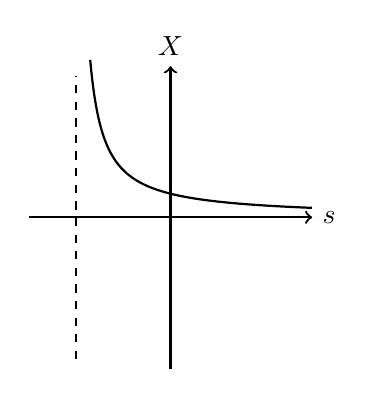
\begin{tikzpicture}[scale=0.6]
    % Parameters
    \def\A{2.828}    % 2sqrt(2)
    \def\a{-0.9}       % alpha
    \def\xMax{3}
    % Axes
    \draw[->,thick] (-3,0) -- (3,0) node[right] {$s$};
    \draw[->,thick] (0,-3.2) -- (0,3.2) node[above] {$X$};

    % Actual function
    \draw[thick,domain=-1.7:\xMax,samples=400]
        plot (\x,{1/(\x+2)});
    \draw[dashed] (-2,-3) -- (-2,3);
\end{tikzpicture}
\caption{$X(s)=\frac{1}{s+2}$}
  \end{subfigure}
  \label{fig:main}
  \caption{A comparison of the original function $x(t)$ and its transform $X(s)$.}
\end{figure}
Notice that the original function $x(t)$ is defined on the time axis $t$, while the transform $X(s)$ is defined on a completely different axis $s$. 
%%%%%%%%%%%%%%%%%%%%%%%%%%%%%%%%%%%%
\subsection{Shorthand}
It isn't necessary to rewrite improper integrals as the limit of a definite integral. We understand that an infinity symbol in the limit corresponds to a limit. For example, we can formally compute the transform of 7:
$$
\mathcal{L}[7] = \int_0^\infty7e^{-st}dt = \left[-\frac{7}{s}e^{-st}\right]_0^\infty=(0)-\left(-\frac{7}{s}\right)=\frac{7}{s},\; \text{when }s>0.
$$
%%%%%%%%%%%%%%%%%%%%%%%%%%%%%%%%%%%%

\begin{example}[3]{
Compute the Laplace transform of $x(t)=t$ using the definition.
}

Start with the definition 
\[
\mathcal{L}[t]=\int_0^\infty t e^{-st}dt
\]
We must use integration by parts $\int u\,dv = uv - \int v\,du$. Let
\[
u=t
\qquad
dv=e^{-st}dt
\]
Then
\[
du=dt
\qquad
v=-\frac{1}{s}e^{-st}
\]
Apply integration by parts:
\[
\int_0^\infty t e^{-st}dt =
-\frac{t}{s}e^{-st}\Big|_0^\infty
+
\frac{1}{s}\int_0^\infty e^{-st}dt.
\]
Now simplify the equation assuming $s>0$:
\begin{align*}
X(s) &= -\frac{t}{s}e^{-st}\Big|_0^\infty + \frac{1}{s}\int_0^\infty e^{-st}dt\\
&=(0-0)+ \frac{1}{s}\int_0^\infty e^{-st}dt\\
&=(0-0)+ \frac{1}{s}\mathcal{L}[1]\\
&=\frac{1}{s}\left(\frac{1}{s}\right)=\frac{1}{s^2}.
\end{align*}
The tranform of the linear function is
\[
\boxed{\mathcal{L}[t]=\frac{1}{s^2},\quad s>0.}
\]
\end{example}

%%%%%%%%%%%%%%%%%%%%%%%%%%%%%%%%%%%%
\section{Piecewise Functions}
One of the most useful features of the Laplace transform is that it can be used on \textit{discontinuous functions}. We will show an example of taking the transform of a discontinuous piecewise function.

\subsection{Definitions}
A \textbf{piecewise function} is a function of the form
$$
    f(t) = \begin{dcases}
        f_1(t), & \text{if } a \le t < b\\ 
        f_2(t), & \text{if } b \le t < c\\
        f_3(t), & \text{if }c \le t < d
    \end{dcases}
$$
The sub-functions $f_1(t)$, $f_2(t)$, $f_3(t)$ are called \textbf{formulas} and the conditions on the right are called \textbf{cases}. Here is an example:
$$
x(t) =
\begin{dcases}
e^{-2t}, & 0 \le t < 1 \\
0, & t \ge 1
\end{dcases}
$$
This function is initially an exponential decay, but it jumps to zero at $t=1$. So $x(t)$ is globally a discontinuous function. Yet we call $x(t)$ piecewise continuous because the formulas are both continuous functions. You can integrate piecewise functions. Integrating them simply means adding up integrals of formulas over their domains. For example 
$$
\int_a^d f(t) \,dt = \int_a^b f_1(t)\,dt + \int_b^c f_2(t)\,dt + \int_c^d f_3(t)\,dt.
$$

\begin{example}[4]{
Find the Laplace transform of
\[
x(t)=
\begin{cases}
e^{-2t}, & 0\le t<1,\\
0, & t\ge1,
\end{cases}
\]
using the definition.
}
Since the function is zero for $t\ge1$, we have
\[
X(s)=\int_0^1 e^{-2t}e^{-st}\,dt
+\int_1^\infty 0\,dt
=\int_0^1 e^{-(s+2)t}\,dt.
\]
This is an integral of a continuous function over a finite
interval, so it converges for every real $s$.

For $s\ne-2$, integration gives
\[
X(s)=
\left[-\frac{e^{-(s+2)t}}{s+2}\right]_0^1
=\frac{1-e^{-(s+2)}}{s+2}.
\]
For $s=-2$, evaluate the integral directly:
\[
X(-2)=\int_0^1 1\,dt=1.
\]
Therefore,
\[
\boxed{
X(s)=
\begin{cases}
\dfrac{1-e^{-(s+2)}}{s+2}, & s\ne-2,\\[6pt]
1, & s=-2.
\end{cases}
}
\]
\end{example}

\subsection{Visualizing the Transform}

The function $x(t)$ is discontinuous at $t=1$, but its
transform $X(s)$ is continuous. The formula
\[
X(s)=\frac{1-e^{-(s+2)}}{s+2}
\]
appears undefined at $s=-2$. In Example 4, we found
$X(-2)=1$ by evaluating the integral directly.
We can also recover this value by taking a limit.

Direct substitution gives the indeterminate form $0/0$,
so we apply L'Hopital's rule:
\[
\lim_{s\to-2}X(s)
=
\lim_{s\to-2}\frac{\tfrac{d}{ds}(1-e^{-(s+2)})}{\tfrac{d}{ds}(s+2)}
=
\lim_{s\to-2}\frac{e^{-(s+2)}}{1}
=1.
\]
Thus, the graph passes through $(-2,1)$ without a hole
or a vertical asymptote. We can also determine the behavior as $s\to\infty$.
Since $e^{-(s+2)}\to0$, the numerator approaches $1$
while the denominator grows without bound:
\[
\lim_{s\to\infty}X(s)
=
\lim_{s\to\infty}\frac{1-e^{-(s+2)}}{s+2}
=0.
\]
These limits help us sketch the transform.


\begin{figure}[H]
\centering
%-------------------- Original function --------------------
\begin{subfigure}[t]{0.46\linewidth}
\centering
\begin{tikzpicture}[x=1.15cm,y=1.6cm]
    \path[use as bounding box]
        (-0.55,-0.4) rectangle (3.2,1.6);

    % Axes
    \draw[->] (-0.25,0) -- (3,0) node[right] {$t$};
    \draw[->] (0,-0.15) -- (0,1.4) node[above] {$x$};

    % Exponential portion: 0 <= t < 1
    \draw[thick,domain=0:1,samples=100]
        plot (\x,{exp(-2*\x)});

    % Zero portion: t >= 1
    \draw[very thick] (1,0) -- (2.8,0);

    % Discontinuity at t=1
    \draw[thick,fill=white]
        (1,{exp(-2)}) circle (2pt);
    \fill (1,0) circle (2pt);

    \node[below] at (1,0) {$1$};
    \node[left] at (0,1) {$1$};
\end{tikzpicture}
\caption{The input $x(t)$ jumps to zero at $t=1$.}
\end{subfigure}
\hfill
%-------------------- Transform --------------------
\begin{subfigure}[t]{0.50\linewidth}
\centering
\begin{tikzpicture}[x=0.42cm,y=1.6cm]
    \path[use as bounding box]
        (-3.6,-0.4) rectangle (7.7,1.6);

    % Axes
    \draw[->] (-3.4,0) -- (7.3,0) node[right] {$s$};
    \draw[->] (0,-0.15) -- (0,1.4) node[above] {$X$};

    % Guides to (-2,1)
    \draw[densely dashed,gray]
        (-2,0) -- (-2,1) -- (0,1);
    \node[below] at (-2,0) {$-2$};
    \node[right] at (0,1) {$1$};

    % Plot on either side of the removable singularity
    \draw[thick,domain=-2.7:-2.01,samples=100]
        plot (\x,{(1-exp(-(\x+2)))/(\x+2)});
    \draw[thick,domain=-1.99:7,samples=250]
        plot (\x,{(1-exp(-(\x+2)))/(\x+2)});

    % Local expansion avoids division by zero at s=-2
    \draw[thick,domain=-2.01:-1.99,samples=10]
        plot (\x,{1-(\x+2)/2+(\x+2)^2/6});

    \fill (-2,1) circle (2pt);
\end{tikzpicture}
\caption{The transform $X(s)$ is continuous at $s=-2$.}
\end{subfigure}

\caption{A discontinuous input and its continuous
Laplace transform. As $s\to\infty$, $X(s)\to0$.}
\end{figure}
%%%%%%%%%%%%%%%%%%%%%%%%%%%%%%%%%%%%
\section{Linearity}
One of the most important properties of the Laplace transform is that it is
\textit{linear}. This property will allow us to compute transforms of complicated
functions by breaking them into simpler pieces.

\subsection{Linear Operators}
A linear operator is a rule that takes a function as input and produces another
function as output while preserving addition and constant multiplication.
Mathematically, an operator $T$ is \textbf{linear} if
\[
T(af+bg)=aT(f)+bT(g), 
\]
where $f$, $g$ are functions and $a$,$b$ are constants. Many familiar operations in calculus are linear operators. For example:

\textbf{Differentiation}
\[
\frac{d}{dt}(af+bg)=a\frac{df}{dt}+b\frac{dg}{dt}.
\]

\textbf{Integration}
\[
\int (af+bg)\,dt
=
a\int f\,dt + b\int g\,dt.
\]
Laplace transforms also enjoy this property.

\textbf{Laplace Transform}
\[
\boxed{
\mathcal{L}\{af(t)+bg(t)\}
=
a\mathcal{L}\{f(t)\}+b\mathcal{L}\{g(t)\}
}
\]
This follows directly from the linearity of integrals.
\[
\int_0^\infty (af+bg)e^{-st}dt
=
a\int_0^\infty fe^{-st}dt
+
b\int_0^\infty ge^{-st}dt
\]
Once we know the transforms of a few basic functions, linearity allows us to
compute transforms of much more complicated functions without evaluating new
integrals.

\subsection{Table of Transforms}

Here is a table summarizing the transformations we have found so far:
\[
\renewcommand{\arraystretch}{2.7}
\begin{array}{|c|c|c|}
\hline
 &  x(t) & \quad X(s) \quad \\ 
\hline
1. & 1 & \dfrac{1}{s} \\ 
\hline
2. & t & \dfrac{1}{s^2} \\ 
\hline
3. & e^{at} & \dfrac{1}{s-a} \\ 
\hline
\end{array}
\]

These formulas will appear frequently throughout the next two weeks. You will be given these formulas on the exam. You are encouraged to use the table as you work through the homework assignment. Using this table and the linearity of the Laplace transform, we may quickly find the transforms of functions without using the definition.

\begin{example}[5]{
Find the transform of the following functions:
\begin{enumerate}
    \item $x(t)=4e^{-2t}+2t$
    \item $x(t)=3+5t$
\end{enumerate}
}
\begin{enumerate}
    \item Using linearity,
\[
\mathcal{L}[x(t)]
=
4\mathcal{L}[e^{-2t}]
+
2\mathcal{L}[t]
\]
Using the transform formulas
\[
\mathcal{L}[e^{-2t}] = \frac{1}{s+2},
\qquad
\mathcal{L}[t] = \frac{1}{s^2}
\]
we obtain
\[
\boxed{
X(s)=\frac{4}{s+2}+\frac{2}{s^2}.
}
\]
\vspace{4mm}

\item Again, using linearity and the table
\[
\mathcal{L}[x(t)]
=
3\mathcal{L}[1]
+
5\mathcal{L}[t]
=
\boxed{
\frac{3}{s}
+
\frac{5}{s^2}.
}
\]
\end{enumerate}    
\end{example}

\subsection{Next Lecture}
The Laplace transform may seem like a convoluted operator. However, it can be a powerful tool to solve differential equations. In the next lecture, we will begin using the Laplace transform to solve IVPs.




\end{document}